\documentclass[a4 paper]{article}
% Set target color model to RGB
\usepackage[inner=1.5cm,outer=1.5cm,top=2.5cm,bottom=2.5cm]{geometry}
\usepackage{setspace}
\usepackage[rgb]{xcolor}
\usepackage{verbatim}
\usepackage{amsgen,amsmath,amstext,amsbsy,amsopn,tikz,amssymb,tkz-linknodes}
\usepackage{fancyhdr}
\usepackage[colorlinks=true, urlcolor=blue,  linkcolor=blue, citecolor=blue]{hyperref}
\usepackage[colorinlistoftodos]{todonotes}
\usepackage{rotating}
\usepackage{enumitem}
\usepackage{amssymb}


%\usetikzlibrary{through,backgrounds}
\hypersetup{%
pdfauthor={Arman Shokrollahi},%
pdftitle={Homework},%
pdfkeywords={Tikz,latex,bootstrap,uncertaintes},%
pdfcreator={PDFLaTeX},%
pdfproducer={PDFLaTeX},%
}
%\usetikzlibrary{shadows}
\usepackage[francais]{babel}
\usepackage{booktabs}
\newcommand{\ra}[1]{\renewcommand{\arraystretch}{#1}}

      \newtheorem{thm}{Theorem}[section]
      \newtheorem{prop}[thm]{Proposition}
      \newtheorem{lem}[thm]{Lemma}
      \newtheorem{cor}[thm]{Corollary}
      \newtheorem{defn}[thm]{Definition}
      \newtheorem{rem}[thm]{Remark}
      \numberwithin{equation}{section}

\newcommand{\report}[5]{
   \pagestyle{myheadings}
   \thispagestyle{plain}
   \newpage
   \setcounter{page}{1}
   \noindent
   \begin{center}
   \framebox{
      \vbox{\vspace{2mm}
    \hbox to 6.50in { {\bf EC4213/ET5402/CT5303:~Machine learning and deep learning \hfill Fall 2019} }
       \vspace{4mm}
       \hbox to 6.28in { {\Large \hfill #1 \hfill}}
       \vspace{1mm}
       \hbox to 6.28in { {\hfill #2  \hfill} }
       \vspace{3mm}
       \hbox to 6.28in { {\it Instructor: #3 \hfill #4 (#5)}}
      \vspace{2mm}}
   }
   \end{center}
   \markboth{#5 -- #1}{#5 -- #1}
   \vspace*{4mm}
}

\newcommand{\bbF}{\mathbb{F}}
\newcommand{\bbX}{\mathbb{X}}
\newcommand{\bI}{\mathbf{I}}
\newcommand{\bX}{\mathbf{X}}
\newcommand{\bx}{\mathbf{x}}
\newcommand{\bY}{\mathbf{Y}}
\newcommand{\bw}{\mathbf{w}}
\newcommand{\bepsilon}{\boldsymbol{\epsilon}}
\newcommand{\balpha}{\boldsymbol{\alpha}}
\newcommand{\bbeta}{\boldsymbol{\beta}}
\newcommand{\0}{\mathbf{0}}
\DeclareMathOperator*{\argmax}{arg\,max}
\DeclareMathOperator*{\argmin}{arg\,min}
\newcommand\gldec[2]{
\underset{#1}{\overset{#2}{\gtrless}}
}
\usepackage{titlesec}
\titlespacing*{\section}
{1.5em}{1.5em}{1em}
\titlespacing*{\subsection}
{1.5em}{1em}{1em}


\begin{document}
\report{Report for CA2}{}{Jonghyun Choi}{Jwa Younkyung}{20165174}

REPORT1. Report the error. Discuss any ideas to reduce the errors \\
Using my implementation of vanilla linear regression, the MSE(mean squared error) is 38285489834.36369. By standard scaling with normal distribution, error is 0.28161601241260686. For reducing the error, we need to delete some feature (sqft living) because there is related with other features (sqft living = sqft above + sqft basement). If we don't delete that feature, error is 0.607168576563699.  

REPORT2. Sweep gamma from 0.0 to 1.0 (or some other reasonable values), plot a graph (x-axis: gamma, y-axis: accuracy) and discuss the effect of the gamma (especially comparing with vanilla linear when gamma=0.) \\
\begin{figure}[!htb]
    \center{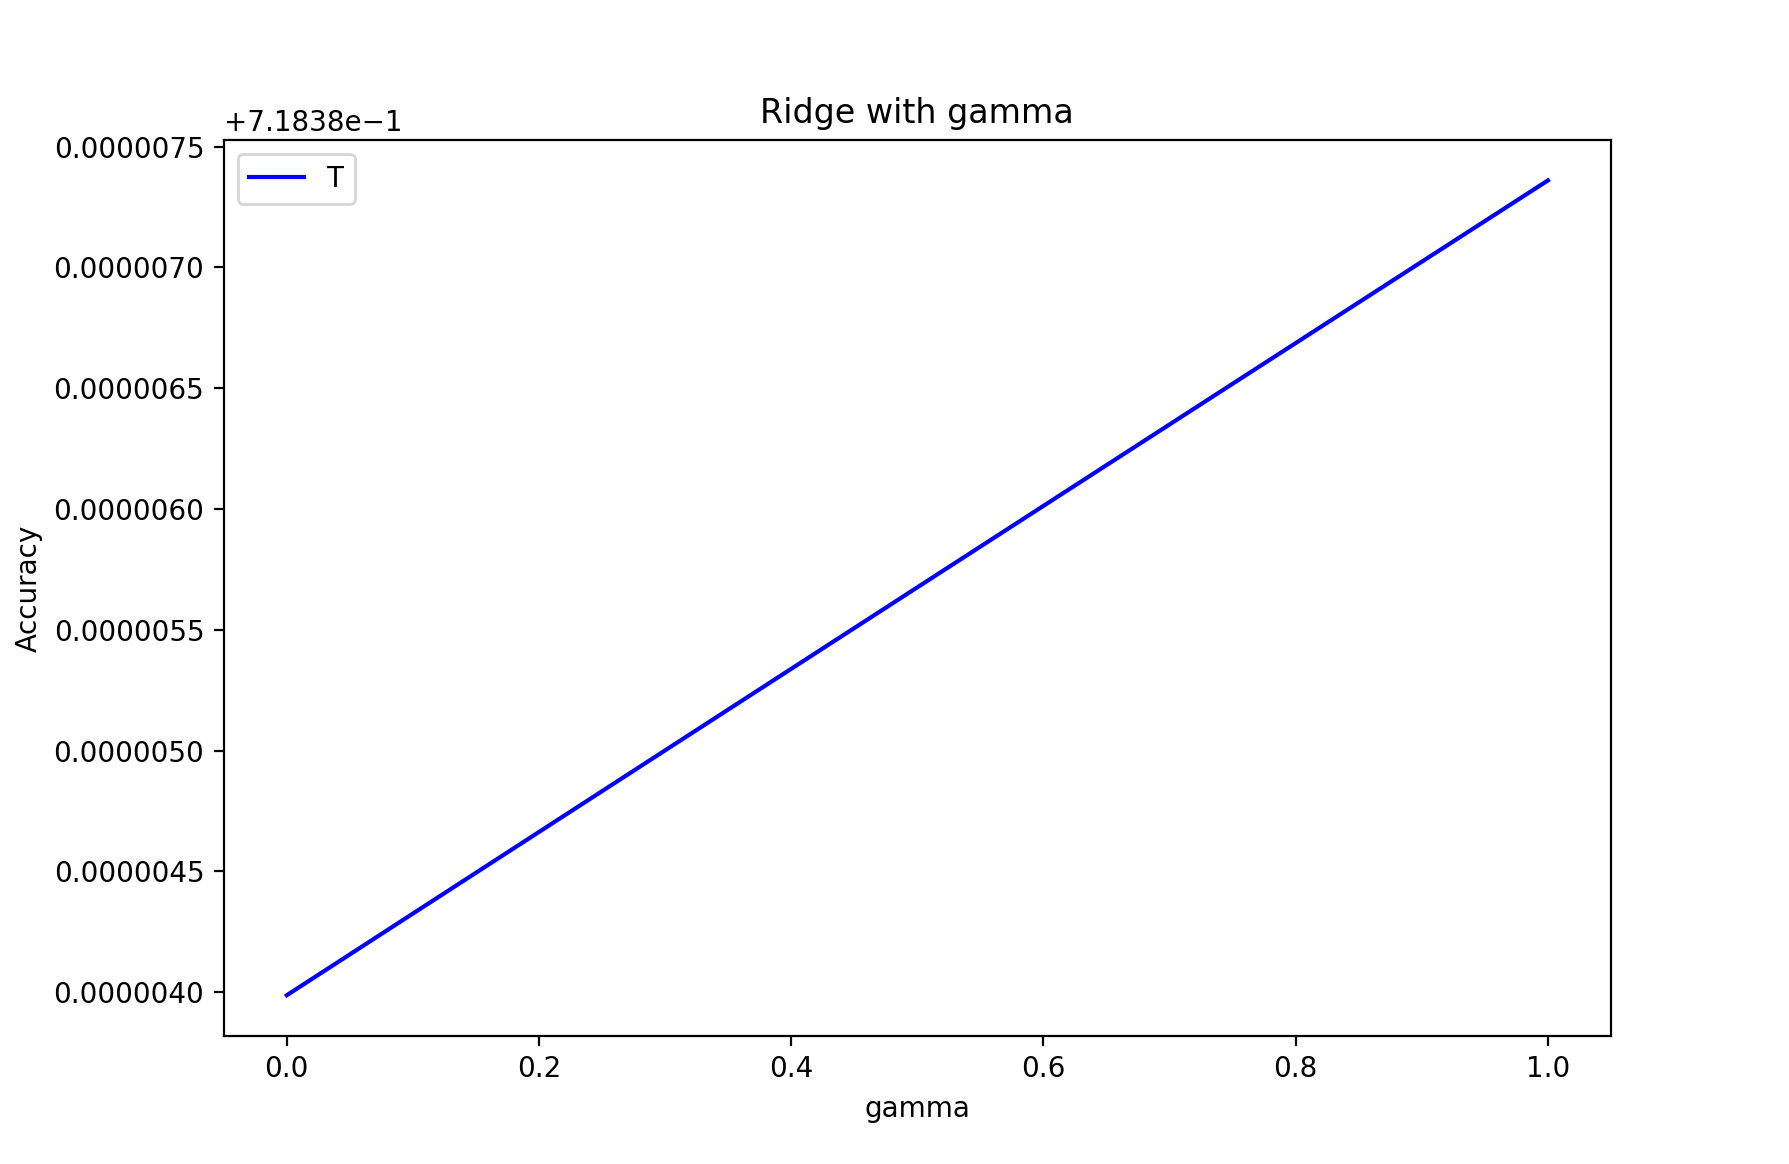
\includegraphics[width=0.5\textwidth]{./ridge_gamma_1.png}}
    \caption{DT on AI.}
    \label{fig:dataset}
\end{figure}

\begin{figure}[!htb]
    \center{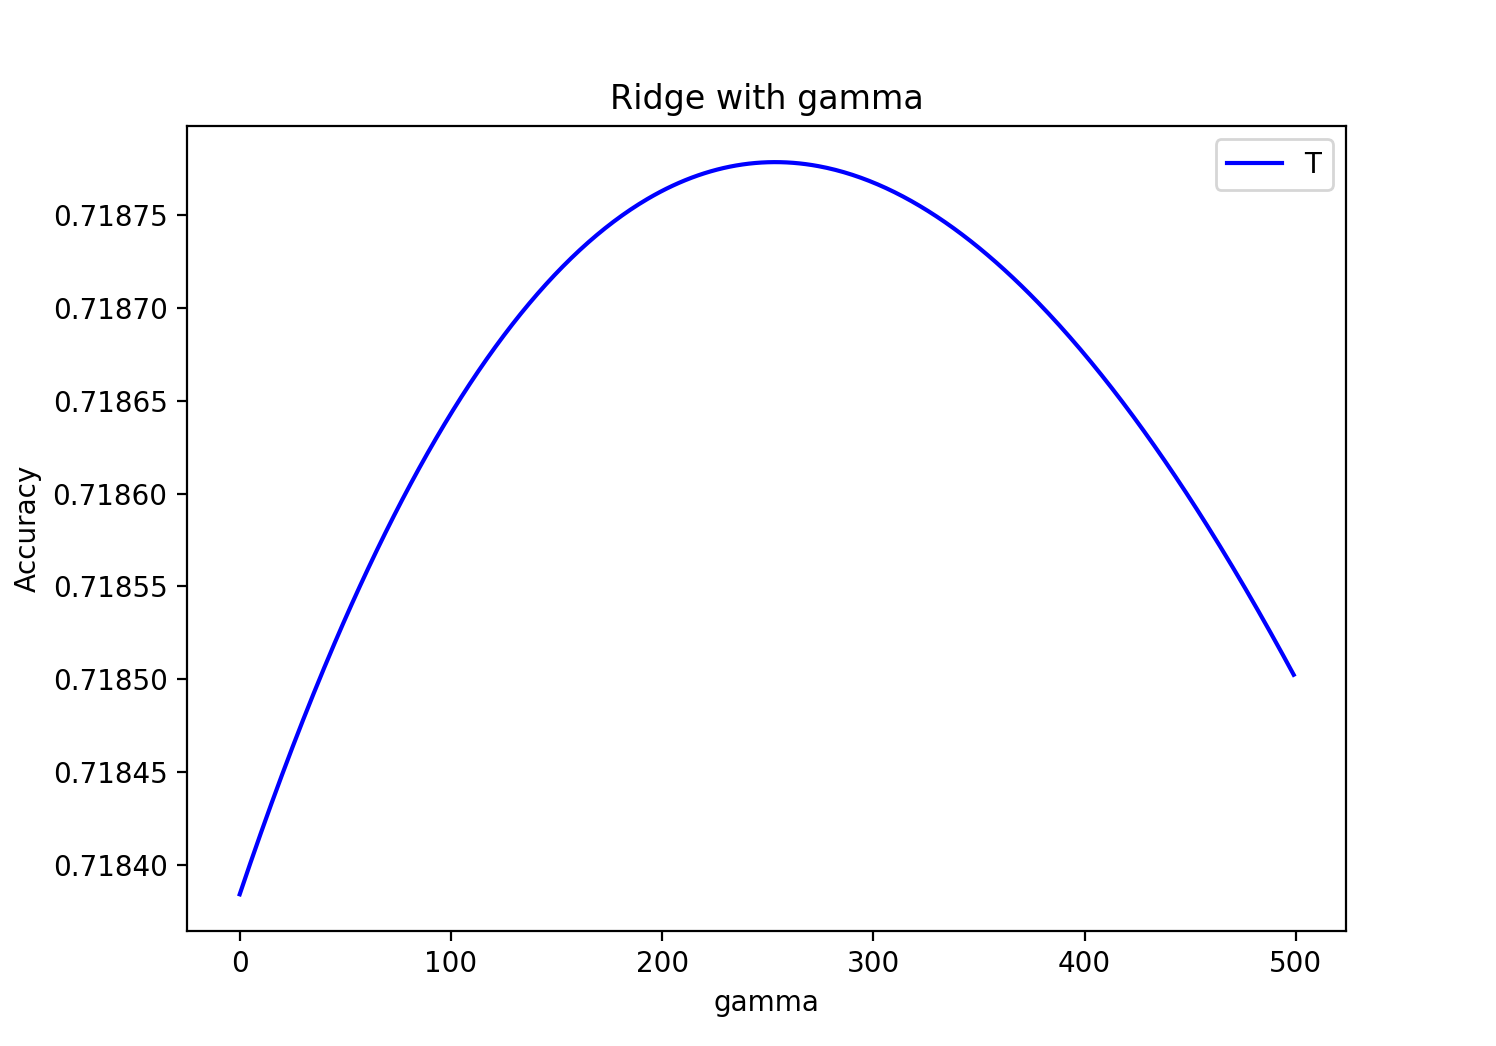
\includegraphics[width=0.5\textwidth]{./ridge_gamma_2.png}}
    \caption{DT on AI.}
    \label{fig:dataset}
\end{figure}
In gamma = 0, the accuracy is about 0.71840. As gamma increases up to about 250, accuracy also increases (about 0.71875). But when gamma is greater than 250, the accuracy decreases. Using gamma can reduce overfitting and penalize.

REPORT4. Report the error. Discuss any improvemental ideas (eg., add regularizers.).

REPORT5. Discuss any idea to solve the regression problem by converting it classification problem.

REPORT6. Compare the error by your implementations of vanilla linear regression and OLS model in scikit-learn and discuss the reason for the difference. If they are identical, report and claim you're awesome! \\
\begin{table}[h]
\begin{tabular}{|c|c|c|}
\hline
error       & non scaling & scaling     \\ \hline
my          & 38285489834 & 0.281616 \\ \hline
scikit      & 38093303528 & 0.281616 \\ \hline
\end{tabular}
\end{table}
My result is very similar with scikit.

REPORT7. Compare the error by your implementations of ridge regression and ridge regression model in scikit-learn and discuss the reason for the difference. If they are identical, report and claim you're awesome! \\
\begin{table}[h]
\begin{tabular}{|c|c|c|}
\hline
error       & non scaling & scaling     \\ \hline
my          & 38284833768 & 0.281612 \\ \hline
scikit      & 38092446800 & 0.281613 \\ \hline
\end{tabular}
\end{table}
My result is very similar with scikit.

REPORT8. Compare the error by your implementations of logistic regression and logistic regression model in scikit-learn and discuss the reason for the difference. If they are identical, report and claim you're awesome!

REPORT9: Discuss all trials you've done with either with your implementations or scikit-learn library's functions.


\end{document}

